\documentclass[conference]{IEEEtran}
\IEEEoverridecommandlockouts
% The preceding line is only needed to identify funding in the first footnote. If that is unneeded, please comment it out.
\usepackage{cite}
\usepackage{amsmath,amssymb,amsfonts}
\usepackage{algorithmic}
\usepackage{graphicx}
\usepackage{textcomp}
\usepackage{xcolor}
\usepackage{subfig}

\usepackage{multirow,array}
\def\BibTeX{{\rm B\kern-.05em{\sc i\kern-.025em b}\kern-.08em
    T\kern-.1667em\lower.7ex\hbox{E}\kern-.125emX}}

\colorlet{dark-cyan}{cyan!75!black}
\newcommand\katja[1]{{\color{dark-cyan}Katja: #1}}

\newcommand\TODO[1]{{\color{red}TODO: #1}}
\newcommand\MAYBE[1]{{\color{blue} #1}}

\begin{document}
\setlength{\intextsep}{0.5ex}

\title{Win or Learn Fast Proximal Policy Optimisation}

\author{\IEEEauthorblockN{Dino Stephen Ratcliffe}
\IEEEauthorblockA{\textit{Electronic Engineering and Computer Science} \\
\textit{Queen Mary University of London}\\
London, England \\
D.Ratcliffe@qmul.ac.uk}
\and
\IEEEauthorblockN{Katja Hofmann}
\IEEEauthorblockA{\textit{Microsoft Research Cambridge} \\
\textit{Microsoft}\\
Cambridge, England \\
Katja.Hofmann@microsoft.com}
\and
\IEEEauthorblockN{Sam Devlin}
\IEEEauthorblockA{\textit{Microsoft Research Cambridge} \\
\textit{Microsoft}\\
Cambridge, England \\
Sam.Devlin@microsoft.com}
}

\maketitle

\begin{abstract}
% draft 1
%    In order to solve many problems agents are required to compete within an environment shared by many other agents. This problem is tackled by multi-agent reinforcement learning (MARL). Treating multi-agent problems as simply non-stationary environments has been shown to produce sub optimal performance. One solution to MARL is to learn a Nash Equilibrium that guarantees a known minimum payoff when playing against other rational agents. We focus on one approach for learning Nash equilibria, Win or Learn Fast (WoLF). WoLF has been shown to converge towards Nash equilibria in a variety of matrix-games and grid based games. We present a systematic empirical investigation into whether WoLF can be effectively adapted to Deep RL, and the characteristics of using WoLF with function approximation. We demonstrate that WoLF is able to improve the performance of Proximal Policy Optimisation (PPO) in multiple environments and give insight into environment properties that help PPO learn strategies close to the Nash Equilibrium.

% draft 2
    AI agents within video games are often required to compete within an environment shared by many other agents. This problem is tackled by multi-agent reinforcement learning (MARL). Applying single agent learning approaches to multi-agent problems has been shown to produce sub-optimal performance due to the environment appearing non-stationary. One solution to MARL is to learn a Nash Equilibrium Strategy (NES) that guarantees a known minimum payoff when playing against other rational agents. We focus on one approach for learning a NES, Win or Learn Fast (WoLF). WoLF has been shown to converge towards a NES in a variety of matrix-games and grid based games. Research into Deep MARL has focused on performance against opponent agents and with limited quantitative results regarding learning a NES. We present a systematic empirical investigation into the ability of Proximal Policy Optimistaion (PPO) to learn a NES, showing instability in certain matrix games. We then present an extension WoLF-PPO, that is able to learn a policy that is closer to the NES.
\end{abstract}

\begin{IEEEkeywords}
    Artificial intelligence, Artificial neural networks, Multi-agent systems
\end{IEEEkeywords}
\section{Introduction}

% draft 1
In multi-agent environments the learning problem is non-stationary due to the fact that the other agents polices are changing over time. Traditional Reinforcement Learning (RL) techniques have guarantees that rely on the problem domain being a Markov Decision Process (MDP), given the multi-agent environment is non-stationary this does not hold and the guarantees are lost. Win or Learn Fast (WoLF) attempts to provide guarantees in these situations\cite{bowling2002multiagent}. It provides guarantees of converging to a NES in theory, and has been shown empirically to get closer to a NES than a fixed learning rate agent. Learning a NES is very desirable as it allows us to learn a stationary policy that has a known lower bound payoff when dealing with rational agents.

In this paper we present an initial study into the ability of PPO to learn the NES in a set of traditional game theory matrix-games. We then present an extension to PPO, WoLF-PPO, that is designed to learn policies closer to the NES. We observe that PPO can learn polices close to the NES when it happens to be the max-entropy policy. We also show that WoLF-PPO is able to learn polices closer to the NES than PPO irrespective of if the NES lies on the NES, as well as being more robust to high learning rates.

\section{Background}

%\subsection{Game Frameworks}

% draft 1
%\subsubsection{Markov Decision Process} is the framework that represents single agent environments. MDP can be represented by the tuple $(\mathcal{S}, \mathcal{A}, \mathcal{T}, \mathcal{R})$ were $S$ is the set of possible states, $A$ is the set of possible actions, $T$ is a transition function of the form $\mathcal{S}\times\mathcal{A}\times\mathcal{S}\rightarrow [0,1]$ that gives a probability distribution over next states after a given action is performed in a given state. Finally $R$ represents a reward function of the form $\mathcal{S}\times\mathcal{A}\rightarrow \mathbb{R}$ that returns a reward when a given action is performed on a given state. This framework presents a problem that can be solved by maximising the discounted future reward with a given discount factor denoted by $\gamma$. All MDPs can be solved with a stationary deterministic policy, this results in the majority of single agent RL work focusing on agents that solve this type of problem without much consideration of how they may perform in a multi-agent environment where a deterministic strategy may not be optimal.

% removed matrix games notation
%These games can be represented by the following tuple $(n, \mathcal{A}_{1...n}, \mathcal{R}_{1...n})$ where $n$ represents the number of agents, $\mathcal{A}_{i}$ represents the actions available to agent $i$ with $A$ representing the joint action between all agents and $\mathcal{R}_{i}$ represents the reward function for agent $i$. The reward function can be represented as a set of $n$ matrices where $n$ is the number of players. 
% draft 1
\subsection{Matrix Games} 
Matrix games are a framework that deals with multiple agents\cite{basar1999dynamic}. There are two forms of matrix games, zero-sum games and general-sum games. Zero-sum games are strictly competitive, were if one of the agents receives a positive reward then the opposing agent receives a negative reward, this can sum to either zero or some other constant. General-sum games do not have this constraint and can have reward matrices that are identical across agents (resulting in strictly cooperative games) or mixed including both collaborative and competitive interactions between agents. When considering what solved means for this framework two properties emerge, they are the Best Response strategy and the NES\cite{basar1999dynamic}. The best response strategy is the optimal strategy against the joint actions of all the other agents. In the case of playing against a set of stationary opponents there will exist a deterministic best response strategy. The NES takes this one step further and states that all agents should be playing a best response against the joint actions of all its respective opponents. This produces a dynamic where an agent playing the NES can not do better by changing strategy whilst the other agents are also playing a NES. This means that the NES is not an optimal strategy against all agents, however it does provide stability by preventing the agent from being exploited by another strategy. NES have also been proven to exist in all zero-sum games (contain a unique Nash equilibrium) and all general sum games, making it a very desirable strategy to be able to learn.

\begin{figure*}[htbp]
    \subfloat[Standard MP, Small learning rate, Note the scale of the y axis.\label{fig:standard-mp-e2}]{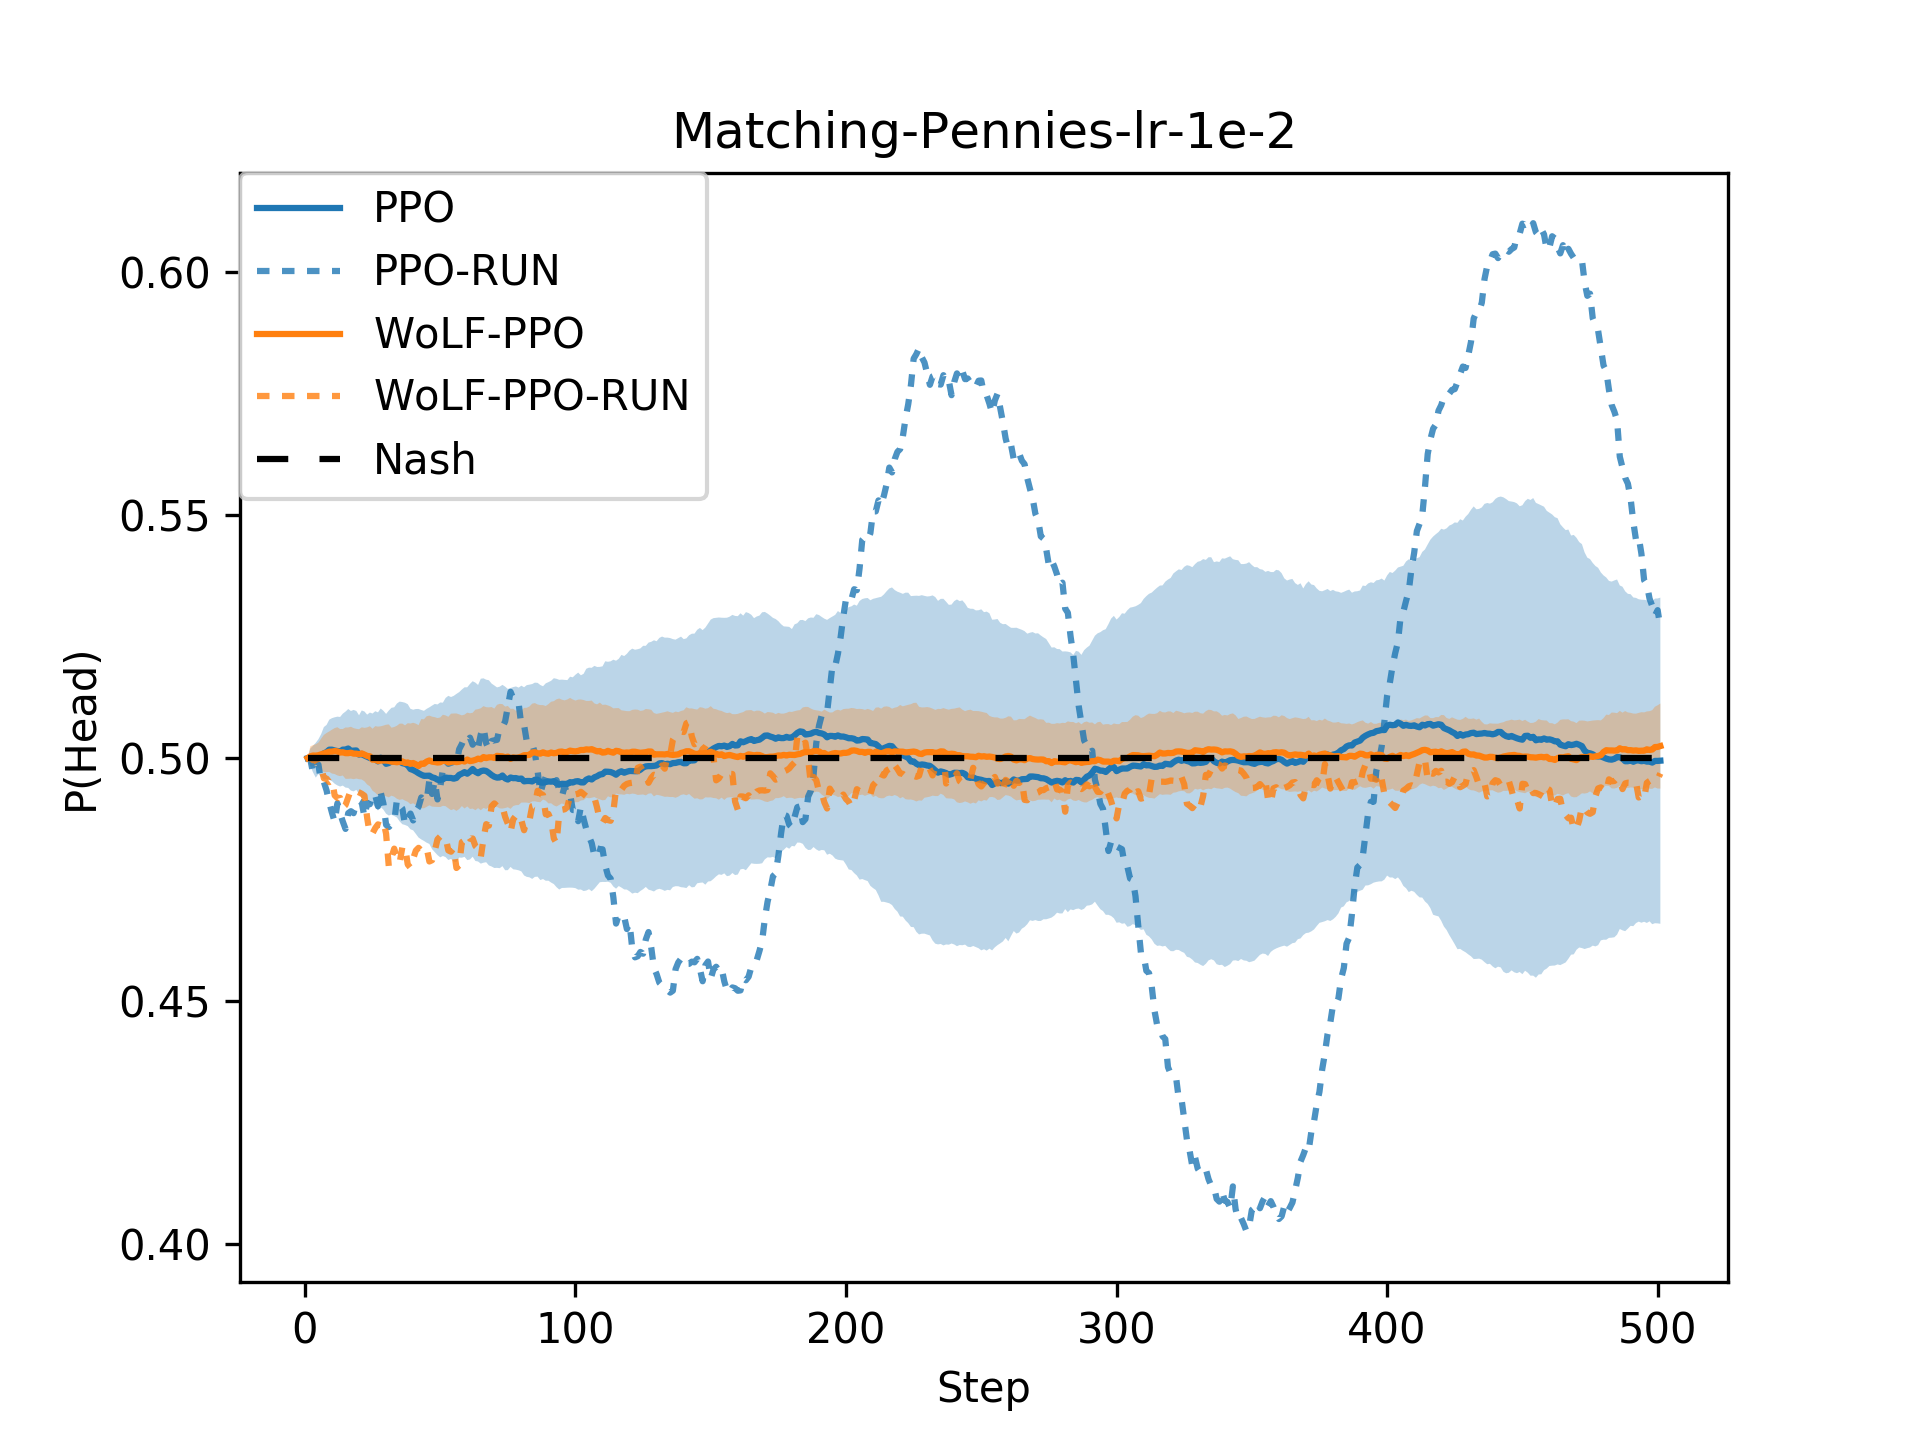
\includegraphics[height=1.8in]{Figures/matching-pennies-lr-1e-2}}
\subfloat[Standard MP, Large learning rate\label{fig:standard-mp-e1}]{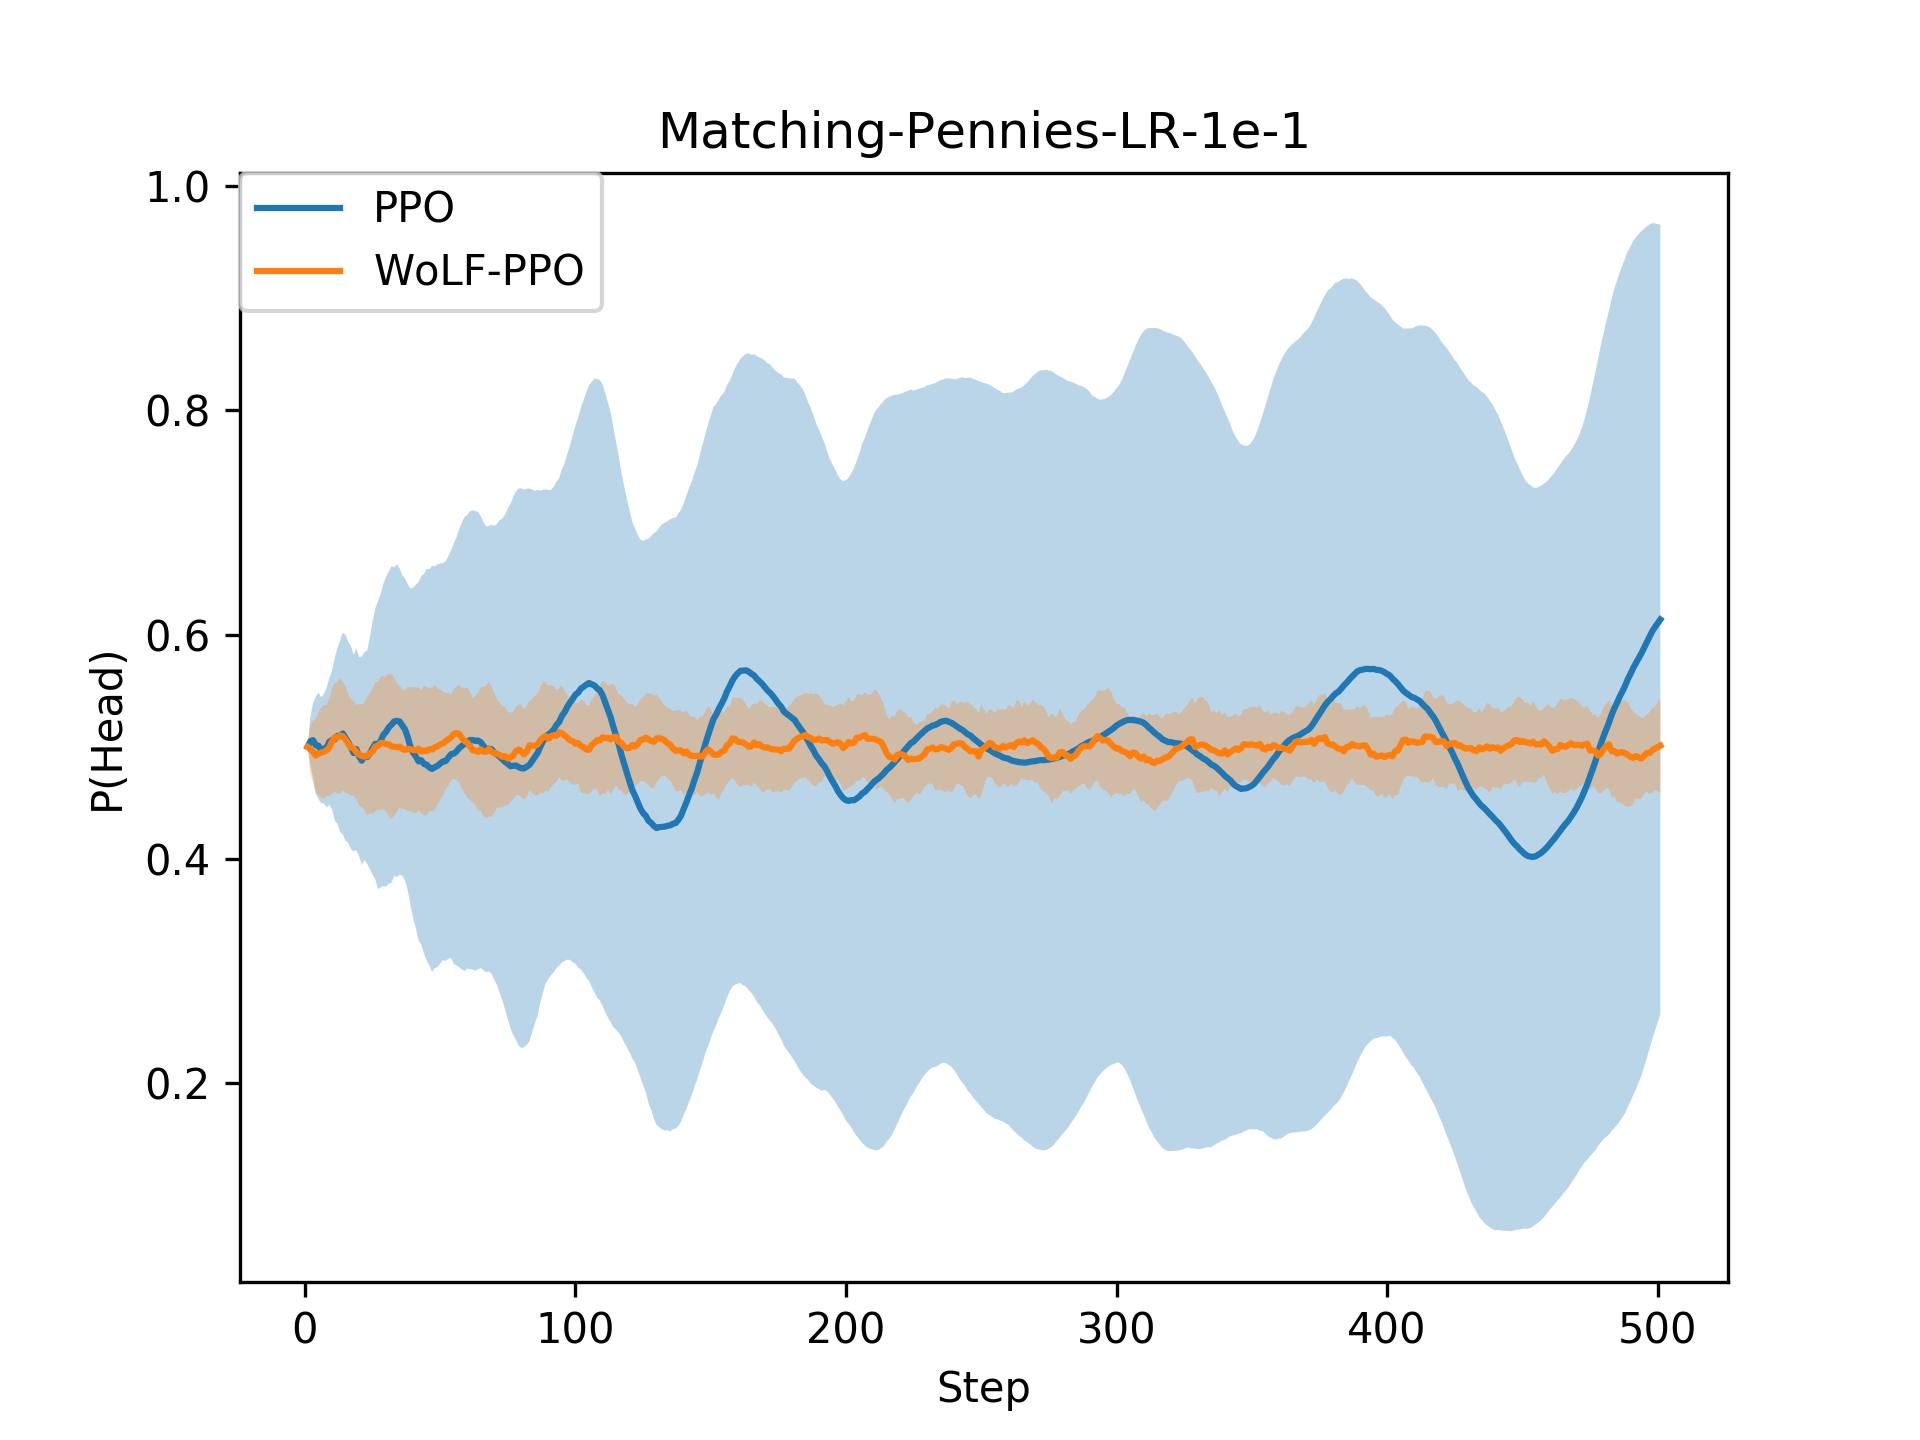
\includegraphics[height=1.8in]{Figures/matching-pennies-lr-1e-1}}
\subfloat[Weighted MP, Small learning rate\label{fig:weighted-mp-e2}]{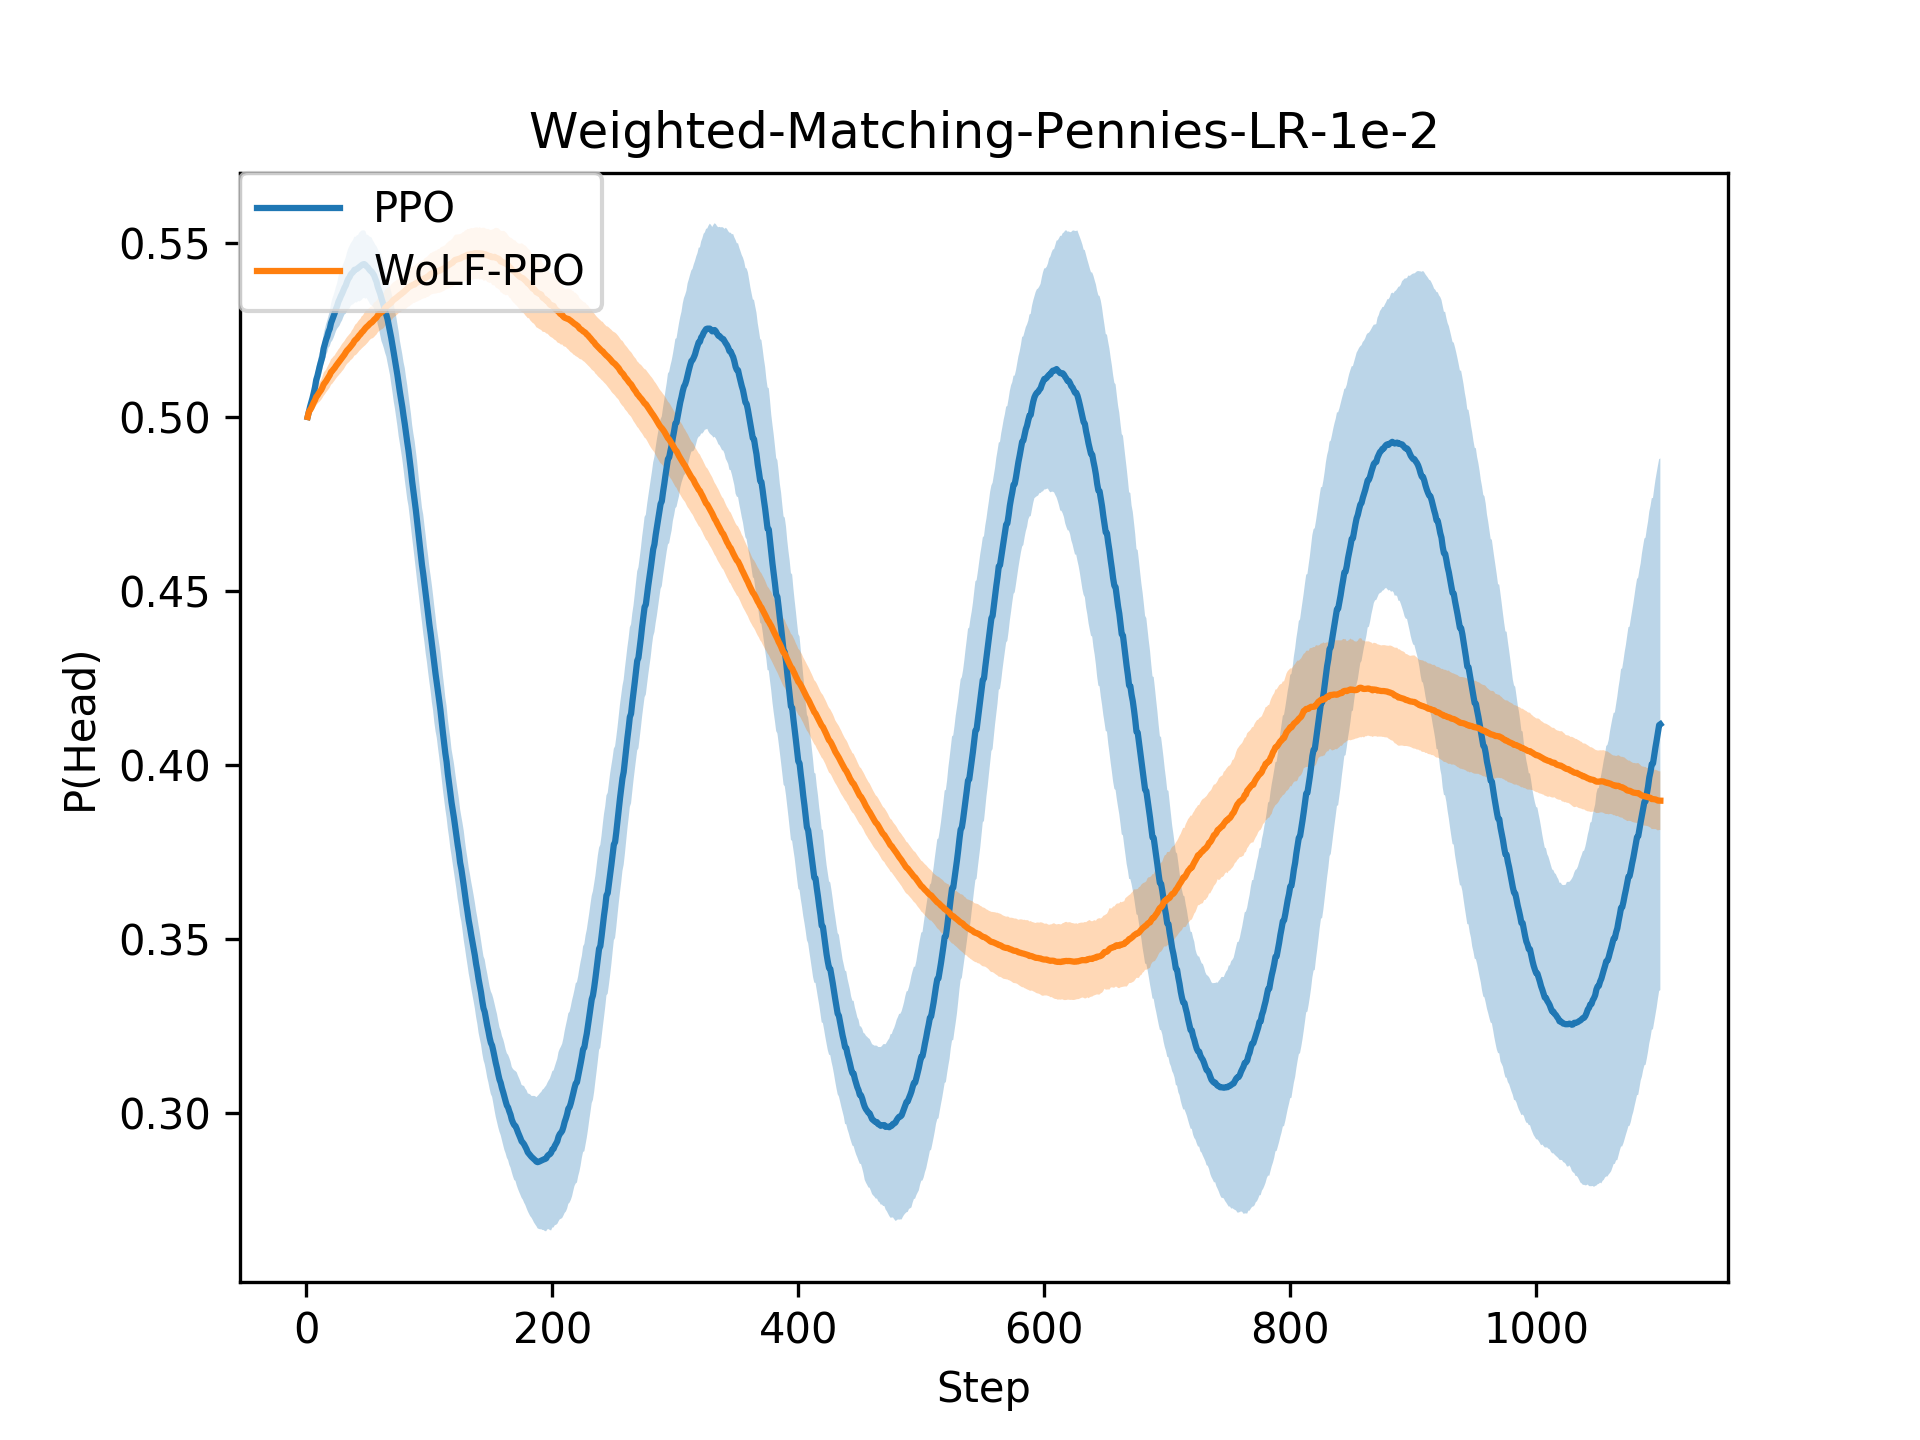
\includegraphics[height=1.8in]{Figures/weighted-matching-pennies-lr-1e-2}}
    \caption{WoLF-PPO vs PPO matching pennies results, $P(Head)$ is the probability of picking head throughout training. Averaged over 50 runs.}
\end{figure*}


%\subsubsection{Stochastic Games} is a frame work that combines the Markov Decision Process (MDP) framework and the 
%Matrix games framework. It can be seen as a MDP with with multiple agents producing 
%a joint action that is used for the transition function and agents reward function. Stochastic games can be seen as the fol owing tuple $(n, \mathcal{S}, \mathcal{A}_{1...n}, 
%\mathcal{T}, \mathcal{R}_{1...n})$. This is with $n$ representing the number of agents 
%in the game, $\mathcal{S}$ being the set of possible states, $\mathcal{A}_{i}$ being the 
%set of actions available to agent $i$, $\mathcal{A}$ represents the set of joint actions, 
%$\mathcal{T}$ is a transition function in the form of 
%$\mathcal{S}\times\mathcal{A}\times\mathcal{S}\rightarrow [0, 1]$ giving a probability 
%distribution over states that result from the joint action $\mathcal{A}$ being performed
%on a given state, finally $\mathcal{R}_{i}$ is a reward function for agent $i$ in the form
%$\mathcal{S}\times\mathcal{A}\rightarrow \mathbb{R}$. As stochastic games are built on MDP and matrix games both of these are subsets of
%stochastic games. A stochastic game with all opposing agents having stationary policies
%is identical to a MDP. If the Stochastic game only has one state then it is identical 
%to a matrix game. Some of the properties from matrix games also transition over to stochastic games, 
%this includes the notion of zero-sum games and general sum games. This also means
%that Nash equilibrium strategies exist for stochastic games and this is the strategy
%that the original WoLF work and our work is trying to learn.
%
%\katja{best response? discuss other solution concepts if relevant}

\subsection{Properties of Multi-Agent systems}

Within the literature two main properties have been identified as desirable for any multi-agent learning systems. The first of these properties is rationality. Rationality states, "\textit{If the other players' policies converge to stationary policies then the learning algorithm will converge to a policy that is a best-response to the other players' policies}"\cite{bowling2002multiagent}. The second property is convergence defined as, "\textit{The learner will necessarily converge to a stationary policy. This property will usually be conditioned on the other agents using an algorithm from some class of learning algorithms}"\cite{bowling2002multiagent}. In practise most literature focuses on self play, however some work has been empirically shown to converge with a small subset of learning agents beyond self play\cite{bowling2002multiagent}. Given these two rules if two agents are both rational and convergent then they will both converge to a stationary best response strategy against each other resulting in having converged to a NES.

%The reason that these two rules have been identified as desirable properties for mulitagent
%systems to possess is how their relationship relates to the Nash equilibrium. This comes from 
%the fact that if both agents are rational and both converge to a stationary policy then they
%must have converged to a Nash equilibrium. This can logically be thought through, if both 
%agents are guaranteed to play best response to a stationary policy then neither of the agents 
%can individually change their strategy in order to increase their payoff. Given this the agents 
%must have then converged to a Nash equilibrium.

\subsection{WoLF}
%Infinitesimal Gradient Ascent (IGA) has been proven in self play will either converge to a Nash equilibrium, or the average payoffs over time will converge in the limit to a Nash Equilibrium\cite{singh2000nash}. This provides an agent that is both rational and convergent. However this is regarded as a week form of convergence as it may only converge to the payoff of a Nash equilibrium in expectation. This work was then expanded on with variable learning rates.

Win or Learn Fast (WoLF) is an extension to Infinitesimal Gradient Ascent (IGA)\cite{singh2000nash} giving a stronger notion of convergent to a NES. This is done by introducing separate learning rates for when the agent is winning and when it is losing. The agent is judged to be winning if their current expected payoff is better than playing the Nash equilibrium. This change has the effect of the winning agent learning slower and being more ``cautious'' about updating its strategy until the other agent has learned to counter the new strategy.

%This approach does place some strict requirements on what knowledge is needed of the game. The method requires the player's own payoff matrix to be known and the policy of the opponent agent. It would also need to know the Nash Equilibrium in order to compute if the agent is currently winning or losing, this however can be computed from the known payoffs\cite{bowling2002multiagent}.

Although the proofs for this method do require knowing detailed information about the environment and opponent, a practical algorithm has been presented. This method is based on PHC and uses a comparison of the current expected payoff to the expected payoff of the current average policy over training. This provides a estimation of the equilibrium policy.

\subsection{Proximal Policy Optimisation}

Proximal Policy Optimisation (PPO) is a policy based gradient method for deep reinforcement learning. It is a current state of the art deep reinforcement learning algorithm that has shown good results on Atari games, MuJoCo control tasks\cite{schulman2017proximal} and DoTA 2\cite{OpenAI_dota}. PPO is based on the ideas introduced with Trust Region Policy Optimisation (TRPO)\cite{schulman2015trust}. PPO introduces clipped probability ratios that can be used as a lower bound estimate of the policy performance. This means that PPO only requires first-order optimisation, making PPO easier to implement and support noisy architectures and parameter sharing.

%It does this whilst trying to solve many problems with TRPO. TRPO is relatively complicated to implement when compared to other Deep RL methods, it is not compatible with architectures involving noise, making dropout unusable, similarly TRPO also doesn't allow for parameter sharing making shared layers between policy and value output impossible as well as training with auxiliary tasks.

%PPO is able to improve these shortcomings of TRPO by introducing clipped probability ratios that can be used as a lower bound estimate of the policy performance. This means that PPO only requires first-order optimisation, making PPO easier to implement and support noisy architectures and parameter sharing. 

The objective function for PPO is shown in equation \ref{eq:ppo-objective}.

\begin{equation}
    L_t^{CLIP+VF+S}(\theta) = \hat{\mathbb{E}}_t\big[L_t^{CLIP}(\theta)-c_1L_t^{VF}(\theta)+c_2S[\pi_{\theta}](s_t)\big]
    \label{eq:ppo-objective}
\end{equation}

$c_1$ and $c_2$ are coefficients. $S$ is the max entropy bonus and $L_t^{VF} = (V_{\theta}(s_t)-V_t^{targ})^2$. Here we can see that PPO has a term in its objective function that rewards higher entropy strategies $c_2S[\pi_{\theta}]$, this is to aid in exploration at the beginning of training in order to prevent the agent from learning an overly deterministic policy before exploring the state space. 

\begin{figure*}[htbp]
    \subfloat[Standard RPS, Small learning rate, note the scale of the axes.\label{fig:standard-rps-e2}]{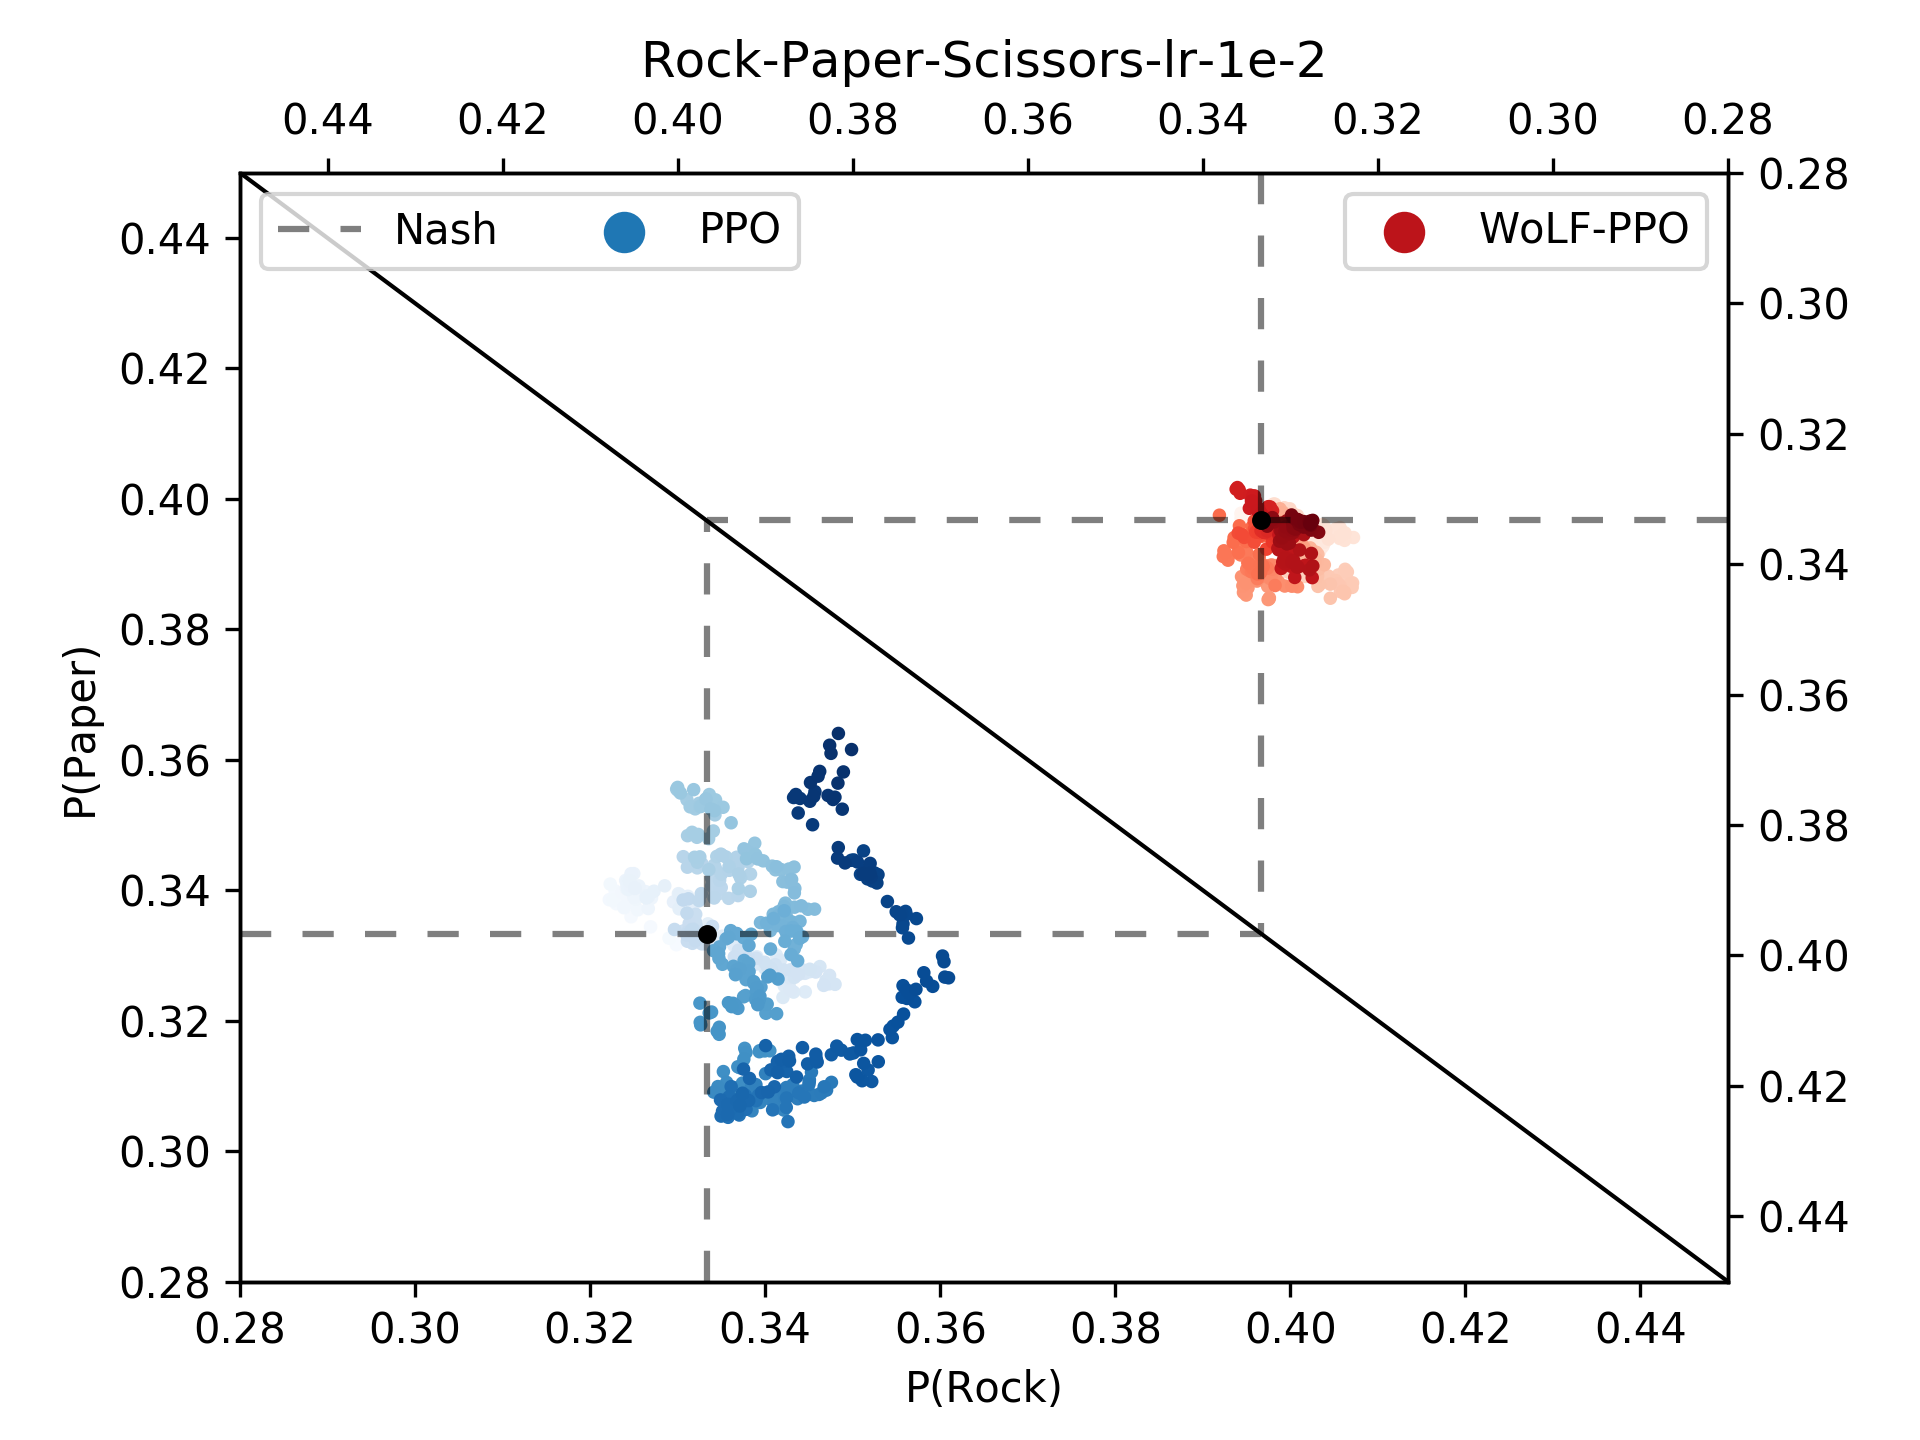
\includegraphics[height=1.8in]{Figures/rock-paper-scissors-lr-1e-2}}
    \subfloat[Standard RPS, Large learning rate\label{fig:standard-rps-e1}]{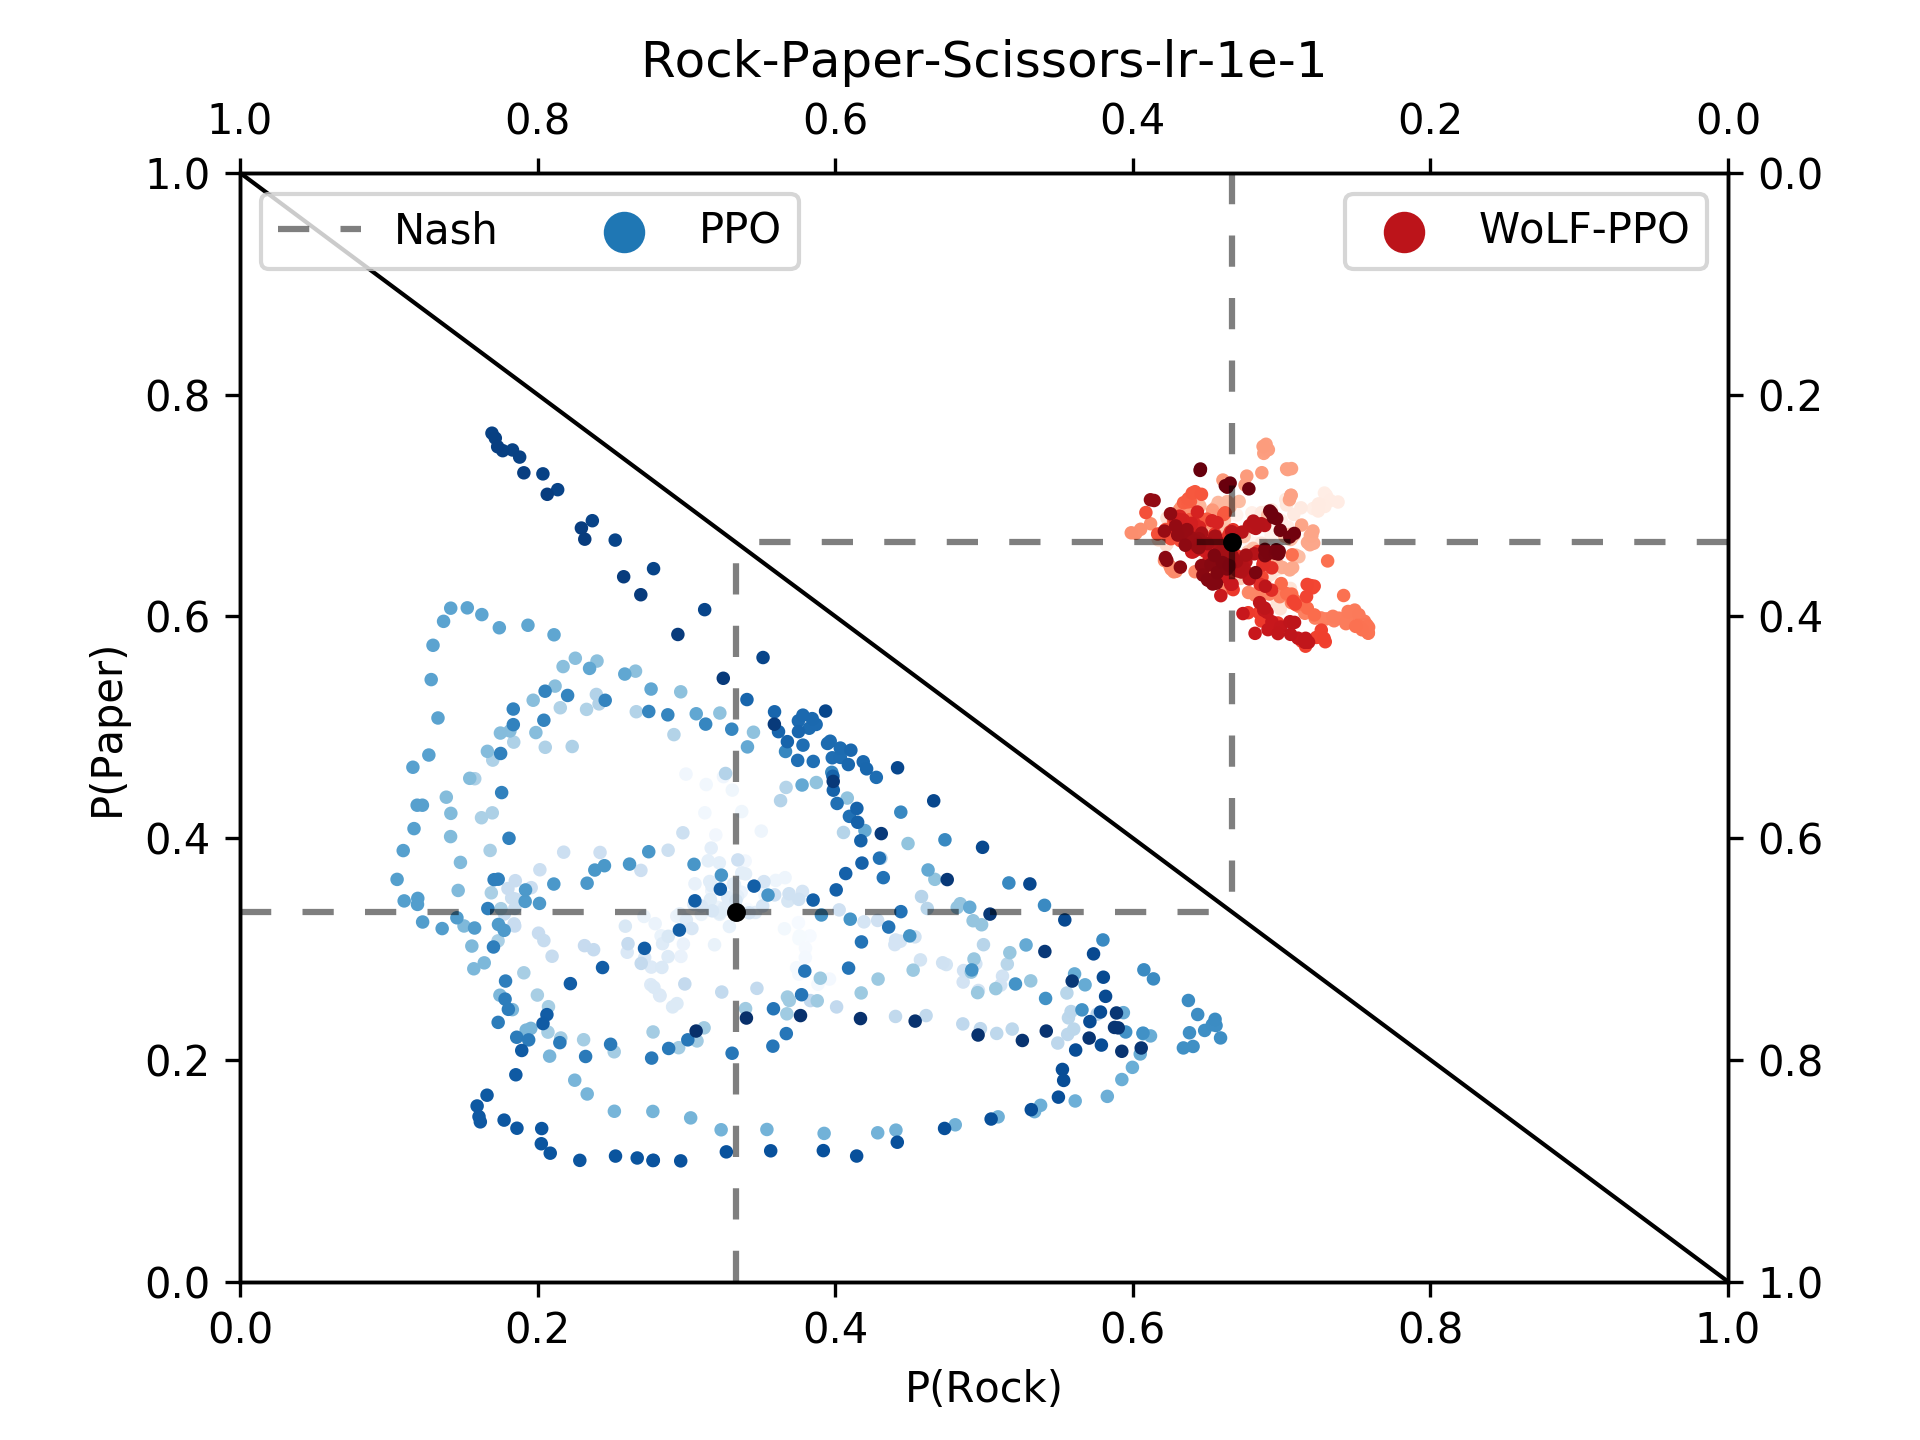
\includegraphics[height=1.8in]{Figures/rock-paper-scissors-lr-1e-1}}
    \subfloat[Weighted RPS, Large learning rate\label{fig:weighted-rps-e1}]{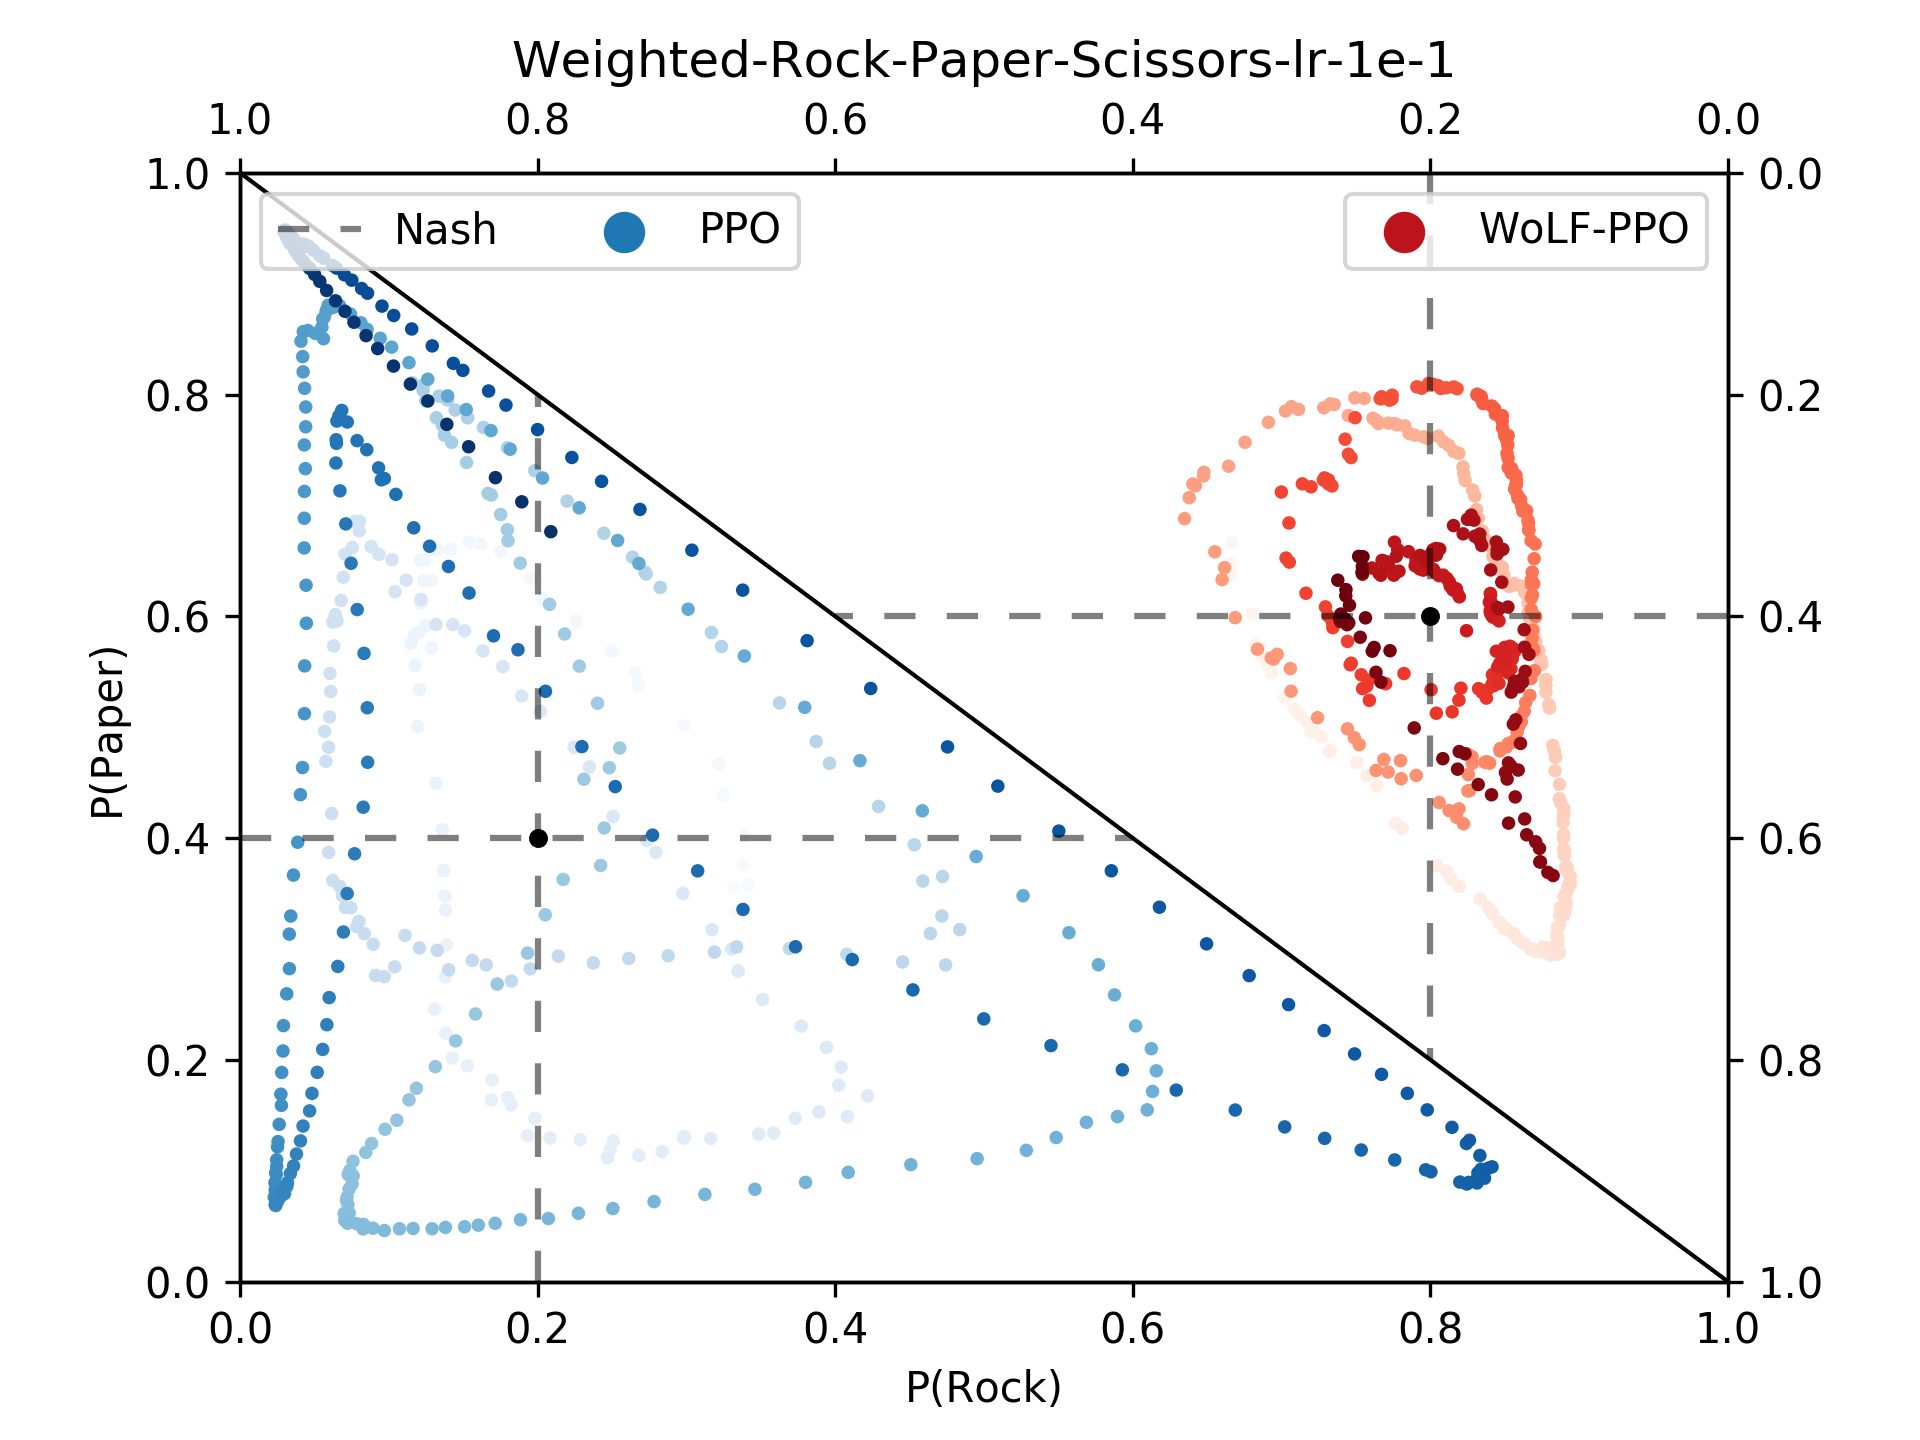
\includegraphics[height=1.8in]{Figures/weighted-rock-paper-scissors-lr-1e-1}}
    \caption{WoLF-PPO vs PPO rock paper scissors results, $P(Rock)$ is the probability of picking rock throughout training, $P(Paper)$ is the probability of picking paper throughout training. Colour transisions from Light to Dark over training steps.}
\end{figure*}


\subsection{Multiagent Policy Gradient Methods}

There has been work attempting to use policy gradient methods in a multi-agent setting. Little work has been done however to evaluate the ability of these systems to learn a NES, instead focusing on performance against other approaches. The work by Lowe et al\cite{lowe2017multi} focuses on performance of actor-critic methods in a range of competitive and cooperative tasks. They present a method that uses extra information at training time with a centralised critic. They also present results for their model when trained with policy ensembles, showing that it improves training stability and agent robustness. However the robustness of the agent is measured by testing the agent against other pre-trained policies. This means that the lower bound for performance is not known for these agents.

In the work by Bansal et al\cite{bansal2017emergent} they evaluate PPO in a variety of complex fully competitive multi-agent control tasks. They observe that during training one agent would often learn to dominate the opponent to the point where the opponent is unable to recover. They introduce opponent sampling in order to give the agents a form of curriculum learning that they state is built into all multi-agent environments. They also observe that the agents final policies vary greatly from run to run with different random seeds. No attempt is made in this work to evaluate the distance from the NES.

\section{Win or Learn Fast Proximal Policy Optimisation (WoLF-PPO)}

% draft 2
When extending an approach to use WoLF two properties are required. Due to the fact that the NES can be stochastic the ability to learn stochastic policies is required. The other property required is that the learning rate of the agent can be varied over training. We chose to use PPO as the base agent as it meets both requirements, along with achieving good results in both single player environments and when training on large sample sizes in complex multi-agent environments\cite{OpenAI_dota}. 

PPO already varies the learning rate as it is annealed over training. In order to extend PPO to WoLF-PPO an estimation of the performance of the NES is needed. In order to do this we average the payoff over training as this will provide an estimation of the payoff the agent would receive when playing the NES. This works well for the games presented but would need to be extended for extensive form games.

In our experiments we used Stochastic Gradient Descent (SGD) as we wanted to avoid interference from the adapting of learning rates introduce by ADAM. We have however observed similar results when using ADAM as the optimiser. For all of our experiments we used a ratio of $4$ between our winning and losing learning rates where $\alpha_{LOSE} = 4\alpha_{WIN}$. The network used for all experiments is a fully connected feed forward neural network, with two hidden layers of $20$ neurons.

\section{Empirical Experiments}


For our empirical results we aimed to highlight the difference between PPO and WoLF-PPO, we have therefore used the same experimental setup and environments from the original WoLF paper, as these were also designed to highlight the advantages of WoLF\cite{bowling2002multiagent}. We also introduce some weighted variants of the environments to highlight the effect of the entropy term present in PPOs objective function. In table \ref{tab:nash-distance} we present quantitative results for the distance from the NES PPO and WoLF-PPO get in the various environments. As the policies will be circling around and through the NES we take the policy that had the furthest distance from the NES in the last 10 policy updates for each run and then average over all 50 runs.

\begin{table}[!h]
    \centering
    \setlength{\extrarowheight}{2pt}
    \begin{tabular}{*{4}{c|}}
      \multicolumn{2}{c}{} & \multicolumn{2}{c}{Player $2$}\\\cline{3-4}
      \multicolumn{1}{c}{} &  & $H$  & $T$ \\\cline{2-4}
      \multirow{2}*{Player $1$}  & $H$ & $(2,-2)$ & $(-1,1)$ \\\cline{2-4}
      & $T$ & $(-1,1)$ & $(1,-1)$ \\\cline{2-4}
    \end{tabular}
    \caption{Payoff matrix for weighted Matching Pennies, with a Nash of $P(H)=0.4$.}
    \label{tab:weighted-mp}
\end{table}

\begin{table*}[t]
    \centering
    \begin{tabular}{l|cc|cc|{c}r}
        \cline{2-5}
        & \multicolumn{2}{ c| }{$\alpha=0.1$} &  \multicolumn{2}{ c| }{$\alpha=0.01$}\\ \cline{1-5}
    \multicolumn{1}{ |l| }{Game}                & PPO & WoLF-PPO & PPO & WoLF-PPO\\
    \hline
        \multicolumn{1}{ |l| }{MP}                  & $0.558 \pm 0.093$ & $\mathbf{0.078 \pm 0.033}$ & $0.056 \pm 0.035$ & $\mathbf{0.012 \pm 0.007}$ \\
        \multicolumn{1}{ |l| }{Weighted MP}         & $0.543 \pm 0.150$ & $\mathbf{0.066 \pm 0.029}$ & $0.113 \pm 0.051$ & $\mathbf{0.085 \pm 0.041}$  \\
        \multicolumn{1}{ |l| }{RPS}                 & $0.476 \pm 0.114$ & $\mathbf{0.078 \pm 0.032}$ & $0.042 \pm 0.021$ & $\mathbf{0.013 \pm 0.007}$  \\
        \multicolumn{1}{ |l| }{Weighted RPS}        & $0.436 \pm 0.120$ & $\mathbf{0.080 \pm 0.040}$ & $0.124 \pm 0.055$ & $\mathbf{0.077 \pm 0.010}$  \\
    \hline
    \end{tabular}
    \caption{Comparison of euclidean distance from NES across approaches, learning rates and games. Mean and Standard Deviation over 50 runs, Max distance taken over last 10 policy updates.}
    \label{tab:nash-distance}
\end{table*}


\subsection{Matching Pennies (MP)}

Matching pennies is a game were both players pick a side of a coin, either heads or tails, these choices are then reveled simultaneously with one player receiving a point if they match and the other receiving a point if they differ. This results in the NES being uniform random, if you pick the side of the coin at random then you will win 50\% of the games irrespective of your opponents strategy. The payoff matrix for the weighted variant is shown in Table \ref{tab:weighted-mp} this variant shifts the NES away from uniform random.

Starting with PPO and WoLF-PPO on the standard weighting of matching pennies we can see that both agents stay close to the NES as shown in Fig \ref{fig:standard-mp-e2} and Table \ref{tab:nash-distance}. In this setting we see that WoLF-PPO does get closer to the NES than PPO but both agents learn strategies close to the NES with PPO within $0.056$ and WoLF-PPO within $0.035$.

When the learning rate is increased by an order of magnitude as in Fig \ref{fig:standard-mp-e1}, it is apparent that the distance from the NES increases for both PPO and WoLF-PPO, however WoLF-PPO stays much closer to the NES with PPO being within $0.558$ and WoLF-PPO being $0.078$. We believe that the relatively good performance of PPO in this environment is due to the maximizing of entropy in PPOs objective function. In games such as matching pennies the NES is to play uniform random and thus max entropy. That results in this version of matching pennies having its NES directly optimized by the max entropy term in the objective function.

We demonstrate this phenomenon by using the weighted variant of Matching Pennies to push the NES away from the max entropy policy. In Fig \ref{fig:weighted-mp-e2} we can see that PPO now wildly diverges away from the NES increasing from a distance of $0.056$ away from the NES to $0.113$, with the distance being larger than when dealing with the non weighted matching pennies. We also see that WoLF-PPO continues to outperform PPO by on average learning a strategy within $0.085$ of the NES.

\subsection{Rock Paper Scissors (RPS)}

Rock Paper Scissors (RPS) consists of three possible actions that form a cyclic winning pattern. This environment is of interest becauase in many commercial video games relative skill is non-transitive similar to the dynamics of RPS (e.g. StarCraft\cite{balduzzi2019open}). We again use the standard version of RPS and a weighted variant to move the NES away from uniform random. The payoff matrix for the weighted version can be found in Table \ref{tab:weighted-rps}.

\begin{table}[!ht]
    \centering
    \setlength{\extrarowheight}{2pt}
    \begin{tabular}{*{5}{c|}}
      \multicolumn{2}{c}{} & \multicolumn{2}{c}{Player $2$}\\\cline{3-5}
      \multicolumn{1}{c}{} &  & $R$  & $P$ & $S$ \\\cline{2-5}
      \multirow{2}*{Player $1$}  & $R$ & $(0,0)$ & $(-1,2)$ & $(1,-2)$ \\\cline{2-5}
      & $P$ & $(2,-1)$ & $(0,0)$ & $(-1,1)$ \\\cline{2-5}
      & $S$ & $(-2,1)$ & $(1,-1)$ & $(0,0)$ \\\cline{2-5}
    \end{tabular}
    \caption{Payoff matrix for weighted Rock Paper Scissors, with a Nash of $P(ROCK)=0.2$ and $P(PAPER)=0.4$.}
    \label{tab:weighted-rps}
\end{table}


In RPS we see very similar results to what we observed in matching pennies. In Fig \ref{fig:standard-rps-e2} we show a sample run of PPO and WoLF-PPO, as shown they both stay close to the NES, as with standard matching pennies the Nash equilibrium lays on the max entropy strategy resulting in relatively good performance from PPO. In Table \ref{tab:nash-distance} we can see that PPO was within $0.042$ and WoLF-PPO was within $0.013$ of the NES on average over 50 runs. When increasing the learning rate by an order of magnitude we end up with WoLF-PPO showing a greater advantage over PPO as was the case with matching pennies, shown in Fig \ref{fig:standard-rps-e1}.

We then ran PPO and WoLF-PPO on a weighted version of RPS. This is to move the NES away from the max entropy policy. In Fig \ref{fig:weighted-rps-e1} and Table \ref{tab:nash-distance} we show that in this environment WoLF-PPO stays closer to the NES than PPO. This is consistent with the matching pennies results.

\section{Conclusion}

% Connection with IPD - hysteretic agents ... questions around assessing "winning" or "losing" in more general games

In this paper we present an initial study into the ability of PPO to learn the NES in a set of traditional game theory matrix-games. We then present an extension to PPO, WoLF-PPO, that is designed to learn policies closer to the NES. We demonstrate that PPO is able to learn policies close to the NES when it is the max-entropy policy. We also shown that WoLF-PPO is able to learn a strategy closer to the NES than PPO in a set of matrix games including games where the NES is not the max-entropy policy. In our experiments we showed that the performance of PPO in both standard MP and RPS is better than originally expected. We believe this is due to the fact that the NES for these games lies on the max-entropy policy. PPO contains a max-entropy term in its objective function, resulting in the NES being directly optimised by this additional term. When training on variants of MP and RPS to shift the NES away from the max-entropy policy we observe that WoLF now provides a much greater advantage over traditional PPO as the agent now learns a policy much closer to the NES. It is important to note that using a max-entropy term when training is a popular technique for promoting exploration and preventing agents from committing to a sub optimal strategy early in training. It is used in approaches such as PPO\cite{schulman2017proximal}, TRPO\cite{schulman2015trust} and ACER\cite{Wang2017SampleEA}. We suspect that similar observations could be made with these approaches with the agents performing much better when the max entropy policy is a NES. We also observed that WoLF-PPO is more robust than PPO when dealing with large learning rates. In the future we would like to expand on this work and move to extensive form games. We would then like to expand beyond what is possible with tabular RL in order to demonstrate both the advantages of WoLF and Deep RL by training on games from raw pixel state representations.

%In this work we have demonstrated that the WoLF approach can be extended to Deep RL while providing benefits when learning in multi-agent environments, getting closer to the NES. We would like to expand this to extensive form games in the future. We would then like to expand beyond what is possible with tabular RL in order to demonstrate both the advantages of WoLF and Deep RL by training on raw pixel data.


\bibliography{cog}
\bibliographystyle{ieeetr}

\end{document}
